%--------------- Tangent method ---------

\section{Tangent method} \label{tg}
The method is based on the linear model as described in \cite{doerner1986}. It is recommended only for use with highly plastic materials where the depth of elastic
recovery is less than 10 \% of max.

\begin{figure}[ht]
  \centering
  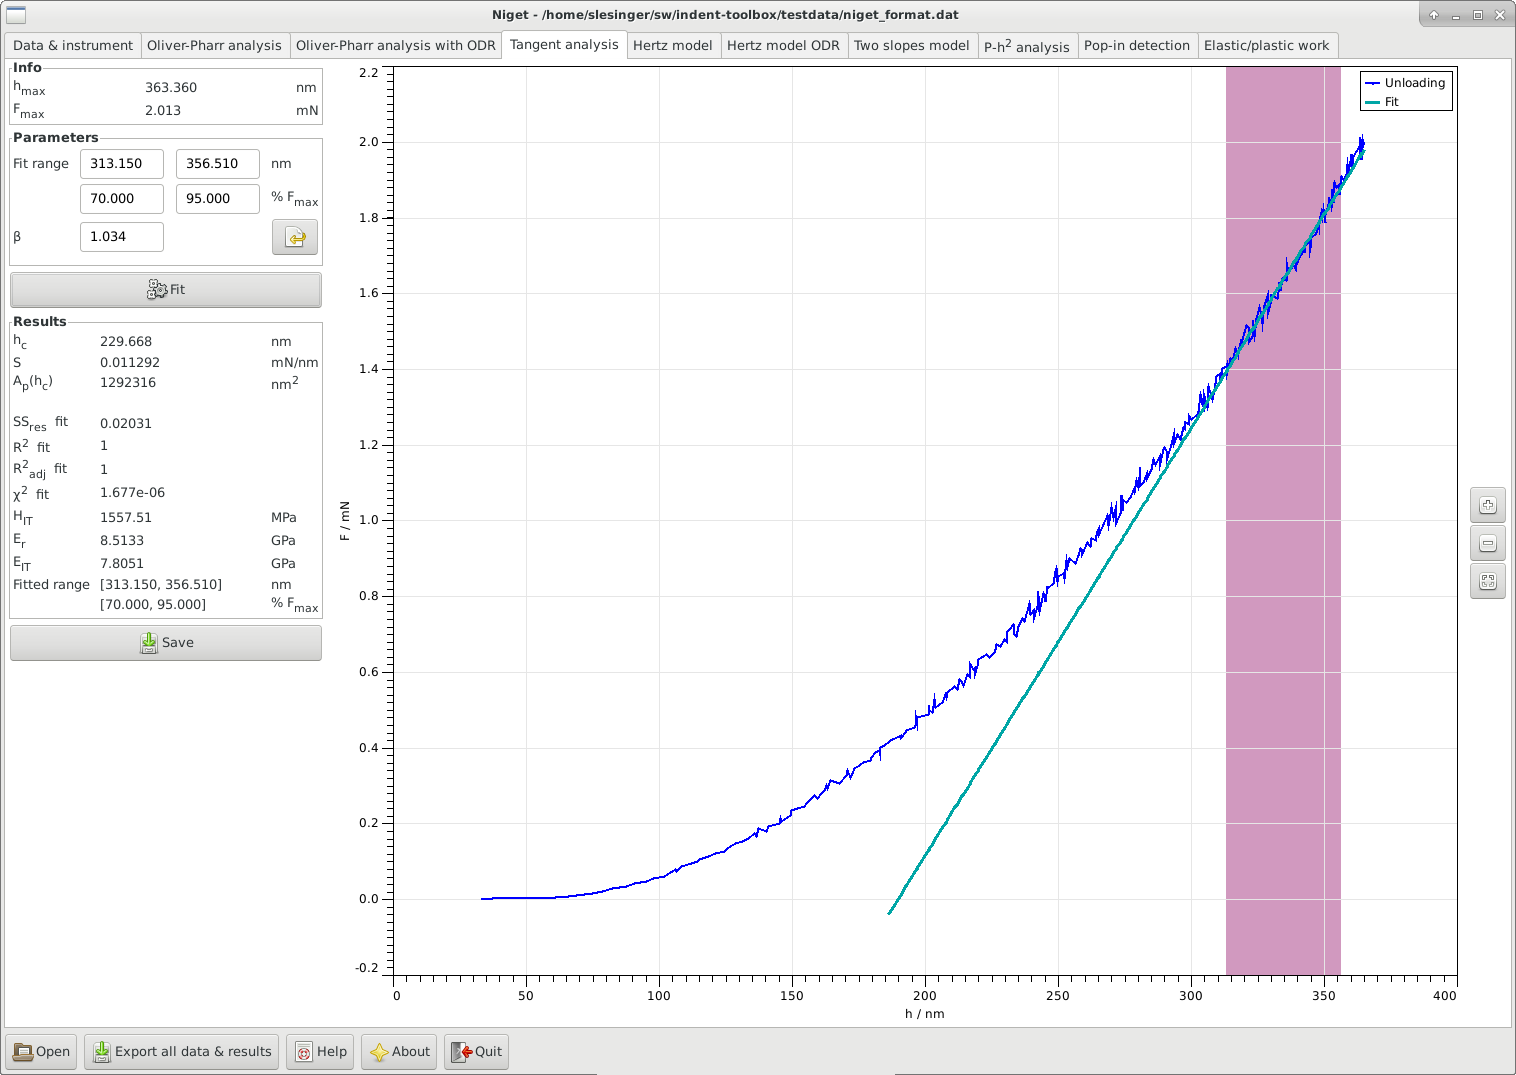
\includegraphics[width=\textwidth]{images/screen-tangent}
  \caption{Tangent method analysis}
\end{figure}


\subsection{Window}
The window consists of several blocks:
\begin{itemize}
 \item \emph{Info} displays the maximum depth and force during the indentation
 \item \emph{Parameters} shows the selected range in nm and in \% of the maximum force, and the correction $\beta$. 
        \begin{itemize}
          \item[-] The fitting range can be selected either using the mouse or typing in the range entries. The range can be defined either in nm or in percent of the maximum force. 
                   It is often recommended to use the range 70--95 \% F$_\mathrm{max}$ for the fit, see section \ref{tg_calc}.  
          \item[-] The parameter $\beta$ accounts for any deviations from the axisymmetric case and is used in the calculation of the reduced modulus in equation \eqref{eq:Er}. 
                   Currently, the default value is the value for three-sided pyramides $\beta = 1.034$. The value supplied by the user is saved in the settings and can be reset to its default value.
        \end{itemize}
 \item \emph{Fit} button, see section \ref{tg_calc} for details of the calculation.
 \item \emph{Results} displays all results in the following order: the contact depth  $\hc$, the slope $S$, the contact area $\Ap(\hc)$, the indentation hardness $H_{IT}$, the contact modulus $E_r$, the indentation modulus $E_{IT}$ and the ranges used for the fitting procedure.
       The variables are described in detail in section \ref{tg_calc}.
 %\item \emph{Uncertainties} show the uncertainty analysis window, see section \ref{tg_unc}.
 \item \emph{Save} save parameters and results to given file. 
 \item \emph{Graph} display the unloading curve and the fitted curves. Stepwise zooming/unzooming can be performed by selecting a range with the mouse and pressing the \emph{Zoom}/ \emph{Unzoom} buttons. The graph is restored to its original size by the \emph{Restore} button.
\end{itemize}

\subsection{Procedure} \label{tg_calc}
The tangent method uses a different approach to determine the slope of the unloading curve at its maximum depth than the Oliver Pharr method.
\begin{enumerate}
 \item Fit the uppermost part of the unloading curve with a straight line using a Deming fit with $\delta = \sigma_F^2/\sigma_h^2$, see section \ref{tls},
 $$
 F = S h + q,
 $$
 using total least squares. The range should be approx. 70--95 \% F$_\mathrm{max}$.
 \item Set $\varepsilon = 0.75$ and calculate the contact depth as
  \begin{equation} \label{eq:hc_tg}
   \hc = \hmax - \varepsilon \Fmax/S.
  \end{equation}

 \item Same as step 4 in \ref{op_calc}.
\end{enumerate}

